\documentclass[pstricks,10pt,dvipsnames]{article} % use larger type; default would be 10pt

\usepackage{enumerate}
\usepackage{hyperref}
\usepackage{amsmath}
\usepackage{ulem}
\usepackage{mathtools}
\usepackage{centernot}
\usepackage{amsfonts}
\usepackage{pgfplots}
\usetikzlibrary{calc,intersections}
\def\Dp{\mathcal{D}'}
\def\R{\mathbb{R}}



\title{Homework 29 (Chap.~14.3),
95.00/120.00 (79.17\%)
}
\begin{document}
\maketitle
\secscore{8}{10}{10}
good
\secscoreFootnote{9}{0}{10}{11,12}
In the problem (a), (b) and (c) are given. What are (1), (2) and (3)?

Also, I disagree with your answer. Suppose (b) is $f$ and consider its section at $x=-2$. The function
looks like.

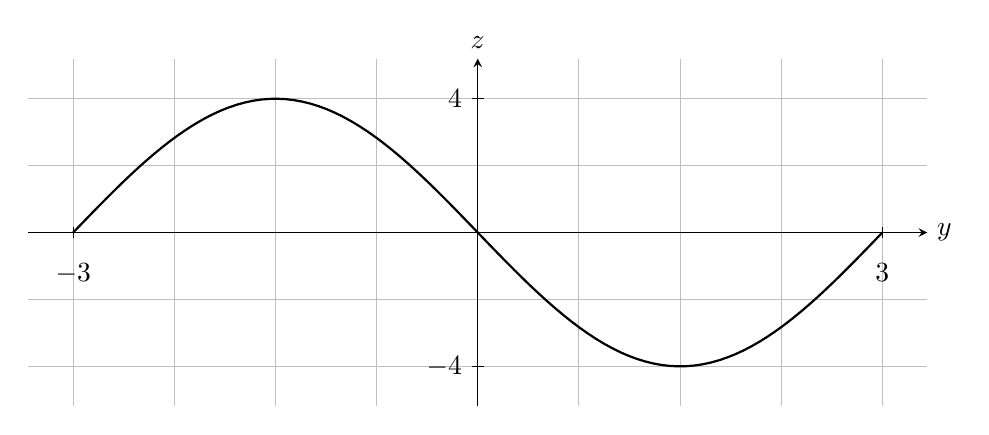
\begin{tikzpicture}
    \begin{axis}[
        height=6cm,
        width=13cm,
        axis lines=middle,
        grid=both,
        domain={-360:360},
        ymin=-1.3, ymax=1.3,
        xmin=-400, xmax=400,
        major tick length=1ex,
        minor tick length=0pt,
        tick style={color=black,thin},
        xtick={-360, 360},
        xticklabels={$-3$, $3$},
        minor xtick={-360,-270,...,360},
        xlabel=$y$,
        every axis x label/.style={
            at={(ticklabel* cs:1)},
            anchor=west,
        },
        xticklabel shift={.2cm},
        ytick={-1,1},
        yticklabels={$-4$, $4$},
        minor ytick={-0.5,0.5},
        ylabel=$z$,
        every axis y label/.style={
            at={(ticklabel* cs:1)},
            anchor=south,
        },
        ]
    \addplot[thick, black, samples=100] { sin(-0.5*x) };
    \end{axis}
\end{tikzpicture}

Hence, the section $x=-2$ of $f_y$ should look like

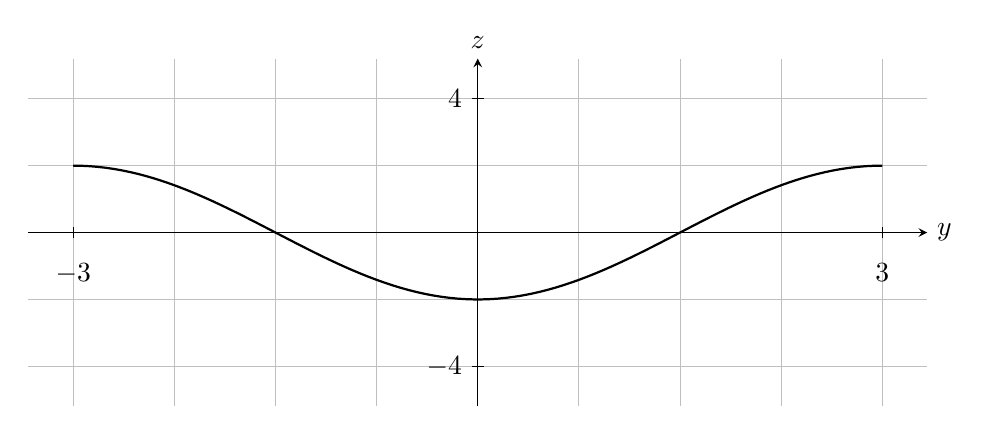
\begin{tikzpicture}
    \begin{axis}[
        height=6cm,
        width=13cm,
        axis lines=middle,
        grid=both,
        domain={-360:360},
        ymin=-1.3, ymax=1.3,
        xmin=-400, xmax=400,
        major tick length=1ex,
        minor tick length=0pt,
        tick style={color=black,thin},
        xtick={-360, 360},
        xticklabels={$-3$, $3$},
        minor xtick={-360,-270,...,360},
        xlabel=$y$,
        every axis x label/.style={
            at={(ticklabel* cs:1)},
            anchor=west,
        },
        xticklabel shift={.2cm},
        ytick={-1,1},
        yticklabels={$-4$, $4$},
        minor ytick={-0.5,0.5},
        ylabel=$z$,
        every axis y label/.style={
            at={(ticklabel* cs:1)},
            anchor=south,
        },
        ]
    \addplot[thick, black, samples=100] { -0.5*cos(-0.5*x) };
    \end{axis}
\end{tikzpicture}

However, it is clearly not so.
\secscore{20}{10}{10}
good
\secscore{30}{10}{10}
good
\secscore{39}{10}{10}
good
\secscore{41}{10}{10}
good
\secscore{45}{10}{10}
good
\secscoreFootnote{50}{5}{10}{51,52}
$\partial z/\partial x$ is good, but in $\partial z/\partial y$
\begin{equation*}
	\frac{z+\frac{x}{y}}{2z-y}\neq\frac{yz-x}{2yz-y^2}\left( =\frac{yz+x}{2yz-y^2} \right).
\end{equation*}
\secscore{60}{10}{10}
good
\secscore{67}{10}{10}
good
\secscore{80}{10}{10}
good
\secscoreFootnote{99}{0}{10}{100,101}
First of all, the section will have an equation $4x^2+z^2=8$. Imagine it plotted in $xz$ plane (with $x$
being horizontal axis and $z$ vertical). Then, point $(x,z)=(1,2)$ is in first quadrant, hence tangent line
should have an equation $x/a+z/b=1$ with $a,b>0$. But you equation is clearly not so.
\end{document}
